\chapter{Determinants}

\section{Commutative Rings}

In this chapter, we define determinants, and we do so for a broader range of matrices, in which its entries are not only from a field but of a more general form, such as polynomials. To do that, we need the following definition.

\begin{definition}[Ring]
	A \textbf{ring}	is a set $K$ together with two operations $+$ (addition) and $\cdot$ (multiplication) satisfying:
	\begin{enumerate}
		\item $K$ is a commutative group under addition;
		\item Multiplication is associative: $(x \cdot y) \cdot z = x \cdot (y \cdot z)$;
		\item The two distributive laws hold: $x \cdot (y + z) = x \cdot y + x \cdot z$ and $(y + z) \cdot x = y\cdot x + z \cdot x$.
	\end{enumerate}
	
	If $x \cdot y = y \cdot x$, then the ring $K$ is said to be \textbf{commutative}.
	
	If there exists an element $e \in K$ such that $e \cdot x = c \cdot e = x$ for each $x \in K$, then $e$ is called the \textbf{identity} for $K$ and the ring $K$ is said to be a \textbf{ring with identity}.
\end{definition}

In this text, we use `ring' to denote a commutative ring with identity.

\section{Determinant Functions}

Intuitively, the determinant has a geometrical meaning: it is an oriented volume. What do we mean by that?

Consider a matrix $A$ and $T_A$ is the transformation that $A$ represents. Notice that the standard basis is a unitary cube, which we denote by $C$. We obtain a parallelepiped by applying the transformation $T_A$ to the unitary cube $C$ (i.e., the standard basis).

So the determinant is the volume of the parallelepiped obtained by the range of the unitary cube by the transformation represented by the matrix.

\begin{figure}[h]
	\centering
	  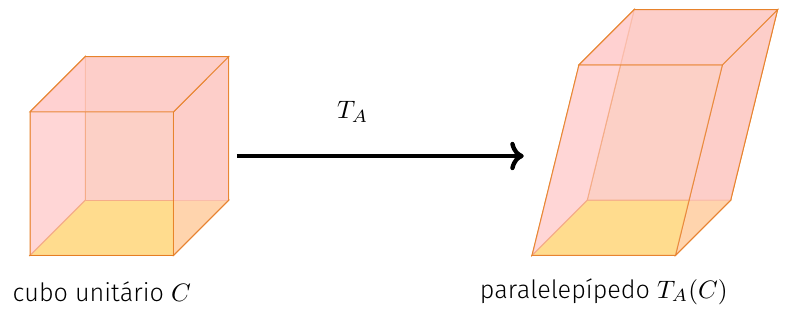
\includegraphics[width=0.8\textwidth]{Figures/geometria_determinante.png} 
	  \caption{The unitary cube $C$ mapped into the parallelepiped $T_A(C)$ \cite{miranda2020avancada}.}
	  \label{fig:geometry-determinant}
\end{figure}

% What properties does this volume must have?

% Volume function: from the square matrices to the field satisfying two simple properties.

% Proposition:

% 1. If a column is zero, then the volume is zero. 

% 2. If the columns are L.D., then the volume is zero.

% 3. Inverting two columns renders $(-1)$ times the original volume. I.e. the volume is alternating (think about permutation groups). 

% 4. Volume is linear in each entry of the matrix (the volume is multilinear).

% Alternating fails at fields of characteristic two. Better way: if two columns are equal, then the volume is zero. Is equivalent to the previous definition and works at $\text{char} ~\textbf{F} = 2$.

% Theorem: A function is a volume volume iff.

% 1. Multilinear;

% 2. Alternating;

% Definition: a function is said to be a determinant if.

% 1. Multilinear;

% 2. Alternating;

% 3. Volume of the unitary cube is one.

% Theorem: uniqueness of the determinant.

Algebraically, our goal is to define a function $\textbf{M}_n(K) \longrightarrow K$ such that it is linear in each row of the matrix (hence it is zero if two rows are equal), and the value of this function applied to the identity matrix is one.

\begin{definition}[$n$-linear]
	Let $K$ be a ring, $n$ a positive integer, and let $D$ be the following function
	\begin{equation*}
		\begin{aligned}
			D : \textbf{M}_n(K) &\longrightarrow K \\
			A &\longmapsto D(A)
		\end{aligned}
	\end{equation*}
	
	Then $D$ is called \textbf{n-linear} if for each $i$, $1 \leq i \leq n$, $D$ is a linear function of the $i$th row when the other $(n-1)$ rows are held fixed.
\end{definition}

Notice that if $v_1, \ldots, v_n$ are the rows of $A$,
\[
	A = \begin{bmatrix}
		\rule{0.7cm}{0.01cm} && v_1 && \rule{0.7cm}{0.01cm} \\
		\rule{0.7cm}{0.01cm} && v_2 && \rule{0.7cm}{0.01cm} \\
		&& \vdots && \\
		\rule{0.7cm}{0.01cm} && v_n && \rule{0.7cm}{0.01cm} \\
	\end{bmatrix}
\]	
Then $D(A)$ is a function of the rows of $A$, i.e.
\[
	D(A) = D(v_1, v_2, \ldots, v_n)
\]

Then $D$ is $n$-linear means that
\[
	D(v_1, \ldots, cv_i + v_i', \ldots, v_n) = cD(v_1, \ldots, v_i, \ldots, v_n) + D(v_1, \ldots, v_i', \ldots v_n)
\]

\begin{example}
	The product of the diagonal entries of an $n \times n$ matrix is $n$-linear.
\end{example}

\begin{lemma}
	A linear combination of $n$-linear functions is $n$-linear.
\end{lemma}

\begin{proof}
	Let $D, E$ be $n$-linears. If $a, b \in K$, then 
	\[
		(aD + bE)(A) = aD(A) + bE(A)
	\]

	Fixing all rows except the $i$th row, we can write $D(v_i)$ instead of $D(A)$. Then 
	\begin{equation*}
		\begin{aligned}
			(aD + bE)(cv_i + v_i') &= aD(cv_i + v_i') + bE(cv_i + v_i') \\
								   &= acD(v_i) + aD(v_i') + bcE(v_i) + bE(v_i') \\
								   &= c(aD + bE)(v_i) + (aD+bE)(v_i')
		\end{aligned}
	\end{equation*}
\end{proof}

\begin{example}
	By the above lemma, the function $D(A) = A_{11}A_{22} - A_{12}A_{21}$ is $2$-linear. 
\end{example}

Notice that for the $D$ defined in the preceding example, we have
\begin{itemize}
	\item $D(I) = 1$;
	\item If two rows are equal, then $D(A) = 0$; 
	\item If $A'$ is obtained from $A$ by interchanging its rows, then $D(A') = - D(A)$, since \[ D(A') = A_{11}'A_{22}' - A_{12}'A_{21}' = A_{21}A_{12} - A_{22}A_{11} = -D(A) \]
\end{itemize}

This fact (plus the geometrical interpretation of volume) induces the following nomenclature.

\begin{definition}[Alternating]
	Let $D$ be a $n$-linear function. We say that $D$ is \textbf{alternating} (or \textbf{alternated}) if the following two conditions are satisfied:
	\begin{enumerate}
		\item $D(A) = 0$ whenever two rows of $A$ are equal;
		\item $D(A') = -D(A)$ if $A'$ is a matrix obt from $A$ by interchanging two rows of $A$.
	\end{enumerate}
\end{definition}

Notice that the second condition fails at fields of characteristic two. But actually, nothing is lost! In fact, the first condition implies the second one. Therefore, we can define alternating functions just using the first condition, which will be equivalent to the previous definition and works at $\text{char} ~\textbf{F} = 2$.

With these tools at hand, we can finally define the determinant.

\begin{definition}[Determinant]
	Let $K$ be a ring, and $n$ a positive integer. Suppose that $D : \textbf{M}_n(K) \longrightarrow K$. Then $D$ is said to be a \textbf{determinant function} if $D$ is $n$-linear, alternating and $D(I) = 1$.
\end{definition}

Our task now is to show the existence and uniqueness of the determinant function.

For $n = 1$, it is trivial: $A = [a]$ and $D(A) = a$.

In the case $n=2$, $D(A)$ is of the form
\[
	D(A) = D(A_{11}e_1 + A_{12}e_2, A_{21}e_1 + A_{22}e_2)
\]

If $D$ is $2$-linear, we have that
\begin{equation*}
	\begin{aligned}
		D(A) &= A_{11}D(e_1, A_{21}e_1 + A_{22}e_2) + A_{12}D(e_2, A_{21}e_1 + A_{22}e_2) \\
		&= A_{11} A_{21} D(e_1, e_1) + A_{11} A_{22} D(e_1, e_2) + A_{12} A_{21} D(e_2, e_1) + A_{12} A_{22} D(e_2, e_2)
	\end{aligned}
\end{equation*}

Hence, $D$ is completely determined by
\[
	D(e_1, e_1), ~D(e_1, e_2), ~D(e_2, e_1), \text{ and } D(e_2, e_2)
\]

We've shown that $D(A) = A_{11}A_{22} - A_{12}A_{21}$ is a determinant function. By the preceeding argument, then $D$ is also unique.

Since $D$ is alternating, 
\[
	D(e_1, e_1) = D(e_2, e_2) = 0
\]
and
\[
	D(e_2, e_1) = - D(e_1, e_2) = -D(I)
\]
and $D(I) = 1$.

\begin{example}
	Let $D$ be any alternating $3$-linear function on $3 \times 3$ matrices over the polynomial ring $\textbf{F}[x]$. And let
	\[
		A = \begin{bmatrix}
			x && 0 && -x^2 \\
			0 && 1 && 0 \\
			1 && 0 && x^3
		\end{bmatrix}
	\]

	Then $D(A) = D(xe_1 - x^2 e_3, e_2, e_1 + x^3e_3)$. Since $D$ is linear in each row,
	\begin{equation*}
		\begin{aligned}
		D(A) &= xD(e_1, e_2, e_1 + x^3 e_3) - x^2D(e_3, e_2, e_1 + x^3 e_3) \\
		&= xD(e_1, e_2, e_1) + x^4D(e_1, e_2, e_3) - x^2D(e_3, e_2, e_1) - x^5D(e_3, e_2, e_3)
		\end{aligned}
	\end{equation*}

	By the hypothesis that $D$ is alternating it follows that
	\[
		D(A) + (x^4 + x^2)D(e_1, e_2, e_3)
	\]
\end{example}

\begin{lemma}
	Let $D$ be a $2$-linear function such that $D(A) = 0$ for all $2 \times 2$ matrices $A$ having equal rows. Then $D$ is alternating.
\end{lemma}

\begin{proof}
	We show that if $A=(u,v)$, then $D(v,u) = -D(u,v)$. Since $D$ is $2$-linear,
	\[
		D(u+v, u+v) = D(u,u) + D(u,v) + D(v,u) + D(v,v) = 0
	\]

	Hence,
	\[
		0 = D(u,v) + D(v,u)
	\]
\end{proof}

\begin{lemma}
	If $D$ is an $n$-linear function and $D(A) = 0$ whenever two adjacent rows of $A$ are equal, then $D$ is alternating.
\end{lemma}

\begin{proof}
	If $A'$ is obtained by interchanging two adjacent rows of $A$, then by the preceeding lemma, $D(A') = -D(A)$. 

	We need to show that $D(A) = 0$ when any two rows of $A$ are equal. Let $B$ be the matrix obtained by interchanging rows $i$ and $j$ of $A$, where $i < j$. We obtain $B$ by a succession of interchanges of pairs of adjacent rows.

	First we interchange the rows $i$ and $i+1$ until the rows are in the order
	\[
		v_1, \ldots, v_{i-1}, v_{i+1}, \ldots, v_j, v_i, v_{j+1}, \ldots, v_n
	\]
	
	This process required $k = j-i$ interchanges of adjacent rows. Now, we need to move $v_j$ to the $i$th position, requiring more $j-1-i = k-1$ interchanges of adjacent rows.

	Since we obtained $B$ from $A$ by $k+(k-1) = 2k-1$ interchanges,
	\[
		D(B) = (-1)^{2k-1}D(A) = -D(A)
	\]

	Now let $A$ be a matrix with two equal rows, say $v_i = v_j$, where $i < j$.
	
	If $j = i+1$, then $D(A) = 0$, since $A$ has two equal and adjacent rows.

	If $j > i+1$, then the batrix $B$, obtained by exchanging the rows $j$ and $i+1$ of the matrix $A$ has two equal and adjacent rows. I.e., $D(B) = 0$.

	Since $D(A) = -D(B)$, then it follows that $D(A) = 0$.
\end{proof}

Next definition and theorem: cofactor method.

\begin{definition}
	If $n>1$ and $A$ is an $n \times n$ matrix, let $A(i|j)$ denote the $(n-1) \times (n-1)$ matrix obtained by deleting the $i$th row and the $j$th row column of $A$. 

	If $D$ is an $(n-1)$-linear function, then we define $D_{ij}(A) = D[A(i|j)]$.
\end{definition}

\begin{theorem}
	Let $n>1$ and $D$ an alternating $(n-1)$-linear function on $(n-1) \times (n-1)$ matrices. For each $j$, where $1 \leq j \leq n$, the function $E_j$ defined by
	\[
		E_j(A) = \sum_{i=1}^n (-1)^{i+j} A_{ij} D_{ij} A
	\]
	is an alternating $n$-linear function on $n \times n$ matrices $A$. If $D$ is a determinant function, so is each $E_j$.
\end{theorem}

\begin{corollary}
	If $K$ is a ring and $n$ is a positive integer, then there exists at least one determinant function on $\textbf{M}_n(K)$.
\end{corollary}

% Determinant and Permutations

% Steps:

% 1. Express every column of the matrix $A$ in terms of the standard basis.

% 2. Using multilinearity, express this as a sum times the determinant of the standard vectors. 

% 3. The repeated terms will vanish, and only the permutations remain.

% If $\sigma$ is the product of $k$ transpositions, then the sign of the determinant will be given by $(-1)^k$. Hence,
% \[
% 	\det (v_1, \ldots, v_n) = \sum_{\sigma \in S_n} \text{sign}(\sigma) v_{\sigma(1)1} v_{\sigma(2)2} \ldots v_{\sigma(n)n}
% \]

% By this formula, we know that the determinant exists.

% Proposition: $\det(A) \neq 0$ iff. $A$ is non-singular.

% Download Jean Dieudonné, Linear algebra and geometry.